%%%%%%%%%%%%%%%%%%%%%%%%%%%%%%% main.tex %%%%%%%%%%%%%%%%%%%%%%%%%%%%%%%
%                                                                      %
% ------------------- Runge-Kutta 4th Order Methods ------------------- %
%                                                                      %
%       Names:                  Email:
%       Kris Melgar Morales      cmelgarmorales@csu.fullerton.edu      %
%       Armanul Ambia            arman714@csu.fullerton.edu            %
%       Angela DeLeo             atakux707@csu.fullerton.edu           %
%       CSUF                                                           %
%       MATH 340-01                                                    %
%%%%%%%%%%%%%%%%%%%%%%%%%%%%%%%%%%%%%%%%%%%%%%%%%%%%%%%%%%%%%%%%%%%%%%%%
%                              Preamble                                %
%%%%%%%%%%%%%%%%%%%%%%%%%%%%%%%%%%%%%%%%%%%%%%%%%%%%%%%%%%%%%%%%%%%%%%%%

% ----------------------------------------------------------------------
% Set the document class
% ----------------------------------------------------------------------
\documentclass[12pt]{article}

% ----------------------------------------------------------------------
% Define external packages, language, margins, fonts, new commands 
% and colors
% ----------------------------------------------------------------------
\usepackage[utf8]{inputenc} % Codification
\usepackage[english]{babel} % Writing idiom

\usepackage[export]{adjustbox} % Align images
\usepackage{amsmath} % Extra commands for math mode
\usepackage{amssymb} % Mathematical symbols
\usepackage{anysize} % Personalize margins
    \marginsize{1in}{1in}{1in}{1in} % {left}{right}{above}{below}
\usepackage{appendix} % Appendices
\usepackage{cancel} % Expression cancellation
\usepackage{caption} % Captions
    \DeclareCaptionFont{newfont}{\fontfamily{cmss}\selectfont}
    \captionsetup{labelfont={bf, newfont}}
\usepackage{cite} % Citations, like [1 - 3]
\usepackage{color} % Text coloring
\usepackage{fancyhdr} % Head note and footnote
    \pagestyle{fancy}
    \fancyhf{}
    \fancyhead[L]{\footnotesize \fontfamily{cmss}\selectfont } % Left of Head note
    \fancyhead[R]{\footnotesize \fontfamily{cmss}\selectfont } % Right of Head note
    \fancyfoot[L]{\footnotesize \fontfamily{cmss}\selectfont CSUF} % Left of Footnote
    \fancyfoot[C]{\thepage} % Center of Footnote
    \fancyfoot[R]{\footnotesize \fontfamily{cmss}\selectfont MATH 340} % Right of Footnote
    \renewcommand{\footrulewidth}{0.4pt} % Footnote rule
\usepackage{float} % Utilization of [H] in figures
\usepackage{graphicx} % Figures in LaTeX
\usepackage[colorlinks = true, plainpages = true, linkcolor = istblue, urlcolor = istblue, citecolor = istblue, anchorcolor = istblue]{hyperref}
\usepackage{indentfirst} % First paragraph
\usepackage[super]{nth} % Superscripts
\usepackage{siunitx} % SI units
\usepackage{subcaption} % Subfigures
\usepackage{titlesec} % Font
    \titleformat{\section}{\fontfamily{cmss}\selectfont\Large\bfseries}{\thesection}{1em}{}
    \titleformat{\subsection}{\fontfamily{cmss}\selectfont\large\bfseries}{\thesubsection}{1em}{}
    \titleformat{\subsubsection}{\fontfamily{cmss}\selectfont\normalsize\bfseries}{\thesubsubsection}{1em}{}
    \fancyfoot[C]{\fontfamily{cmss}\selectfont\thepage}

% Random text (not needed)
\usepackage{lipsum}
\usepackage{duckuments}

\usepackage{url}

% New and re-newcommands
\newcommand{\sen}{\operatorname{\sen}} % Sine function definition
\newcommand{\HRule}{\rule{\linewidth}{0.5mm}} % Specific rule definition
\renewcommand{\appendixpagename}{\LARGE \fontfamily{cmss}\selectfont Appendices}

% Colors
\definecolor{istblue}{RGB}{3, 171, 230}
\definecolor{dkgreen}{rgb}{0,0.6,0}
\definecolor{gray}{rgb}{0.5,0.5,0.5}

%%%%%%%%%%%%%%%%%%%%%%%%%%%%%%%%%%%%%%%%%%%%%%%%%%%%%%%%%%%%%%%%%%%%%%%%
%                                 Document                             %
%%%%%%%%%%%%%%%%%%%%%%%%%%%%%%%%%%%%%%%%%%%%%%%%%%%%%%%%%%%%%%%%%%%%%%%%
\begin{document}
% ----------------------------------------------------------------------
% Cover
% ----------------------------------------------------------------------
\begin{center}
    \mbox{}\\[2.0cm]
    \textsc{\Huge MATH 340}\\[2.5cm]
    \HRule\\[0.4cm]
    {\large \bf {\fontfamily{cmss}\selectfont Runge-Kutta 4th Order Methods -- Lotka-Volterra Equations} [\texttt{EN}]}\\[0.2cm]
    \HRule\\[1.5cm]
\end{center}

\begin{flushleft}
    \textbf{\fontfamily{cmss}\selectfont Authors:}
\end{flushleft}

\begin{center}
    \begin{minipage}{0.5\textwidth}
        \begin{flushleft}
            Kris Melgar Morales \\
            Armanul Ambia \\
            Angela DeLeo 
        \end{flushleft}
    \end{minipage}%
    \begin{minipage}{0.5\textwidth}
        \begin{flushright}
            \href{mailto:cmelgarmorales@csu.fullerton.edu}{\texttt{cmelgarmorales@csu.fullerton.edu}}\\
            \href{mailto:arman714@csu.fullerton.edu}{\texttt{arman714@csu.fullerton.edu}}\\
            \href{mailto:atakux707@csu.fullerton.edu}{\texttt{atakux707@csu.fullerton.edu}}
        \end{flushright}
    \end{minipage}
\end{center}
    
\begin{flushleft}
    \large $\boxed{\text{\bf \fontfamily{cmss}\selectfont Group} \ \clubsuit}$\\[4.0cm]
\end{flushleft}
    
\begin{center}
    \large \bf \fontfamily{cmss}\selectfont 2023 -- Spring Semester
\end{center}

\thispagestyle{empty}

\setcounter{page}{0}

\newpage

% ----------------------------------------------------------------------
% Contents
% ----------------------------------------------------------------------
\tableofcontents 

\newpage

% ----------------------------------------------------------------------
% Body
% ----------------------------------------------------------------------
\section{Introduction}

Predator-prey systems are realistic mathematical models describing the interaction between 2 species, predator and prey, within a closed environment. These systems lend well to differential equations because they are focused on the rate of change of population sizes and how they affect each other. Being able to model the trends of animal populations allows scientists to learn when populations are in danger of becoming extinct or are increasing to unsustainable rates.  

This project analyzes the Lotka-Volterra model, a specific predator-prey system where there are constraints placed on each population. The prey population has access to an infinite food supply and will grow indefinitely without the influence of predators. The predator population starts at a fixed value and will continue to die without the influence of prey. The model uses a pair of equations that generate population densities between predator and prey species at each time step. 
These are the Lotka-Volterra Equations: 
\[\frac{dx}{dt}=\alpha x-\beta xy\]
\[\frac{dy}{dt}=\delta xy- \gamma y\]

\[[\alpha,\beta,\gamma,\delta]\subseteq {\mathbb{R}}_{+}\]

\(\frac{dx}{dt}\) and \(\frac{dy}{dt}\) represent the ``instantaneous growth rates'' of the prey and predator species,
x and y represent ``the population density of prey" and ``some predator", respectively, t represents ``time",
\(\alpha\) is the ``maximum prey per capita growth rate" and \(\beta\) is the predator's effects on the prey population's growth rate,
\(\gamma\) is the ``per capita death rate" of the predator species and \(\delta\) is the prey's effect on the predator growth rate, while ``all parameters are positive and real"\cite{foundation_2023}.

The \(\alpha x\) term represents exponential growth, where the prey is allowed to grow indefinitely ``unless subject to predation". The \(\beta xy\) term is subtracted from the growth term, to represent the rate at which prey die to predators,  determined by the densities of the two populations. \cite{foundation_2023}

The opposing equation defines the instantaneous growth rate of the predator population, where the  \(\delta xy\) represent the ``growth of the predator population" as the predator consumes the prey. The \(\gamma y\) term represents the ``intrinsic death rate" of the predator population.\cite{foundation_2023}.

\newpage

\section{Implementations Details}

In order to generate a graph of population densities from an initial starting point of t = 0 to an arbitrary endpoint,  the Lotka-Volterra equations were solved using the Runge-Kutta Fourth Order Method defined as an algorithm in Section 4 of Chapter 5 of Numerical Analysis\cite{burden_faires_burden_2016}, where 
    
\[a\leq t \leq b\]

\[w_{0} = \alpha \]is the initial condition of the function and
\[k_{1} = hf(t_{i},w_{i}) \]
\[k_{2} = hf(t_{i}+\frac{h}{2},w_{i}+\frac{1}{2}k_{1}) \]
\[k_{3} = hf(t_{i}+\frac{h}{2},w_{i}+\frac{1}{2}k_{2}) \]
\[k_{4} = hf(t_{i+1},w_{i}+k_{3}) \]
\[w_{i+1} = w_{i}+\frac{1}{6}(k_{1}+2k_{2}+2k_{3}+k_{4}) \]
defines the g successive approximation of the list \([w_{0},w_{1},w_{2},...,w_{n}]\) with respect to each time step in the list \([t_{0},t_{1},t_{2},...,t_{n}]\). In our version of this implementation in Matlab, we generated the approximation with a fixed time step method, where \([t_{0},t_{1},t_{2},...,t_{n}]\) is \([0\cdot h,1\cdot h,2\cdot h,..., n\cdot h]\) and h is the size between each step, for a total of n+1 steps in the time interval.  To solve for the Lotka-Volterra equations using the Runge-Kutta Fourth Order function, f is instead treated as a vector of anonymous functions like 

\[\vec{f} = 
\begin{bmatrix}
\frac{dx}{dt}\\ \frac{dy}{dt}
\end{bmatrix}
=
\begin{bmatrix}
\alpha x-\beta xy\\ \delta xy- \gamma y
\end{bmatrix}\]

and \(w_{i}\) is instead a matrix \(w_{ij}\), where each column stores the approximations for each equation, at each time step between the rows, such as initial conditions being stored in 
\[w_{0j} = \begin{bmatrix}
Intitial Prey Density & Intitial Predator Density \\ 
\end{bmatrix} \]


\newpage

\section{Results}

\subsection{Comparison to Matlab Example}
To test the accuracy of our version of the Lotka-Volterra equations using the Runge-Kutta \nth{4} Order method, we plotted a Population Vs Time graph of our method vs the method provided by the Matlab documentation for Predator-Prey Equations\cite{ODE45} using these initial conditions and parameters for the equations.
\[w_{0j} = \begin{bmatrix}
20 & 20 \\ 
\end{bmatrix} \]
\[\vec{f} = 
\begin{bmatrix}
\frac{dx}{dt}\\ \frac{dy}{dt}
\end{bmatrix}
=
\begin{bmatrix}
\alpha x-\beta xy\\ \delta xy- \gamma y
\end{bmatrix}\]
\[0\leq t \leq 15\]
\[h = 1/300, n + 1 = 4500\]



\subsubsection{Matlab Plot Results}

\begin{figure}[H]
        \begin{center}
            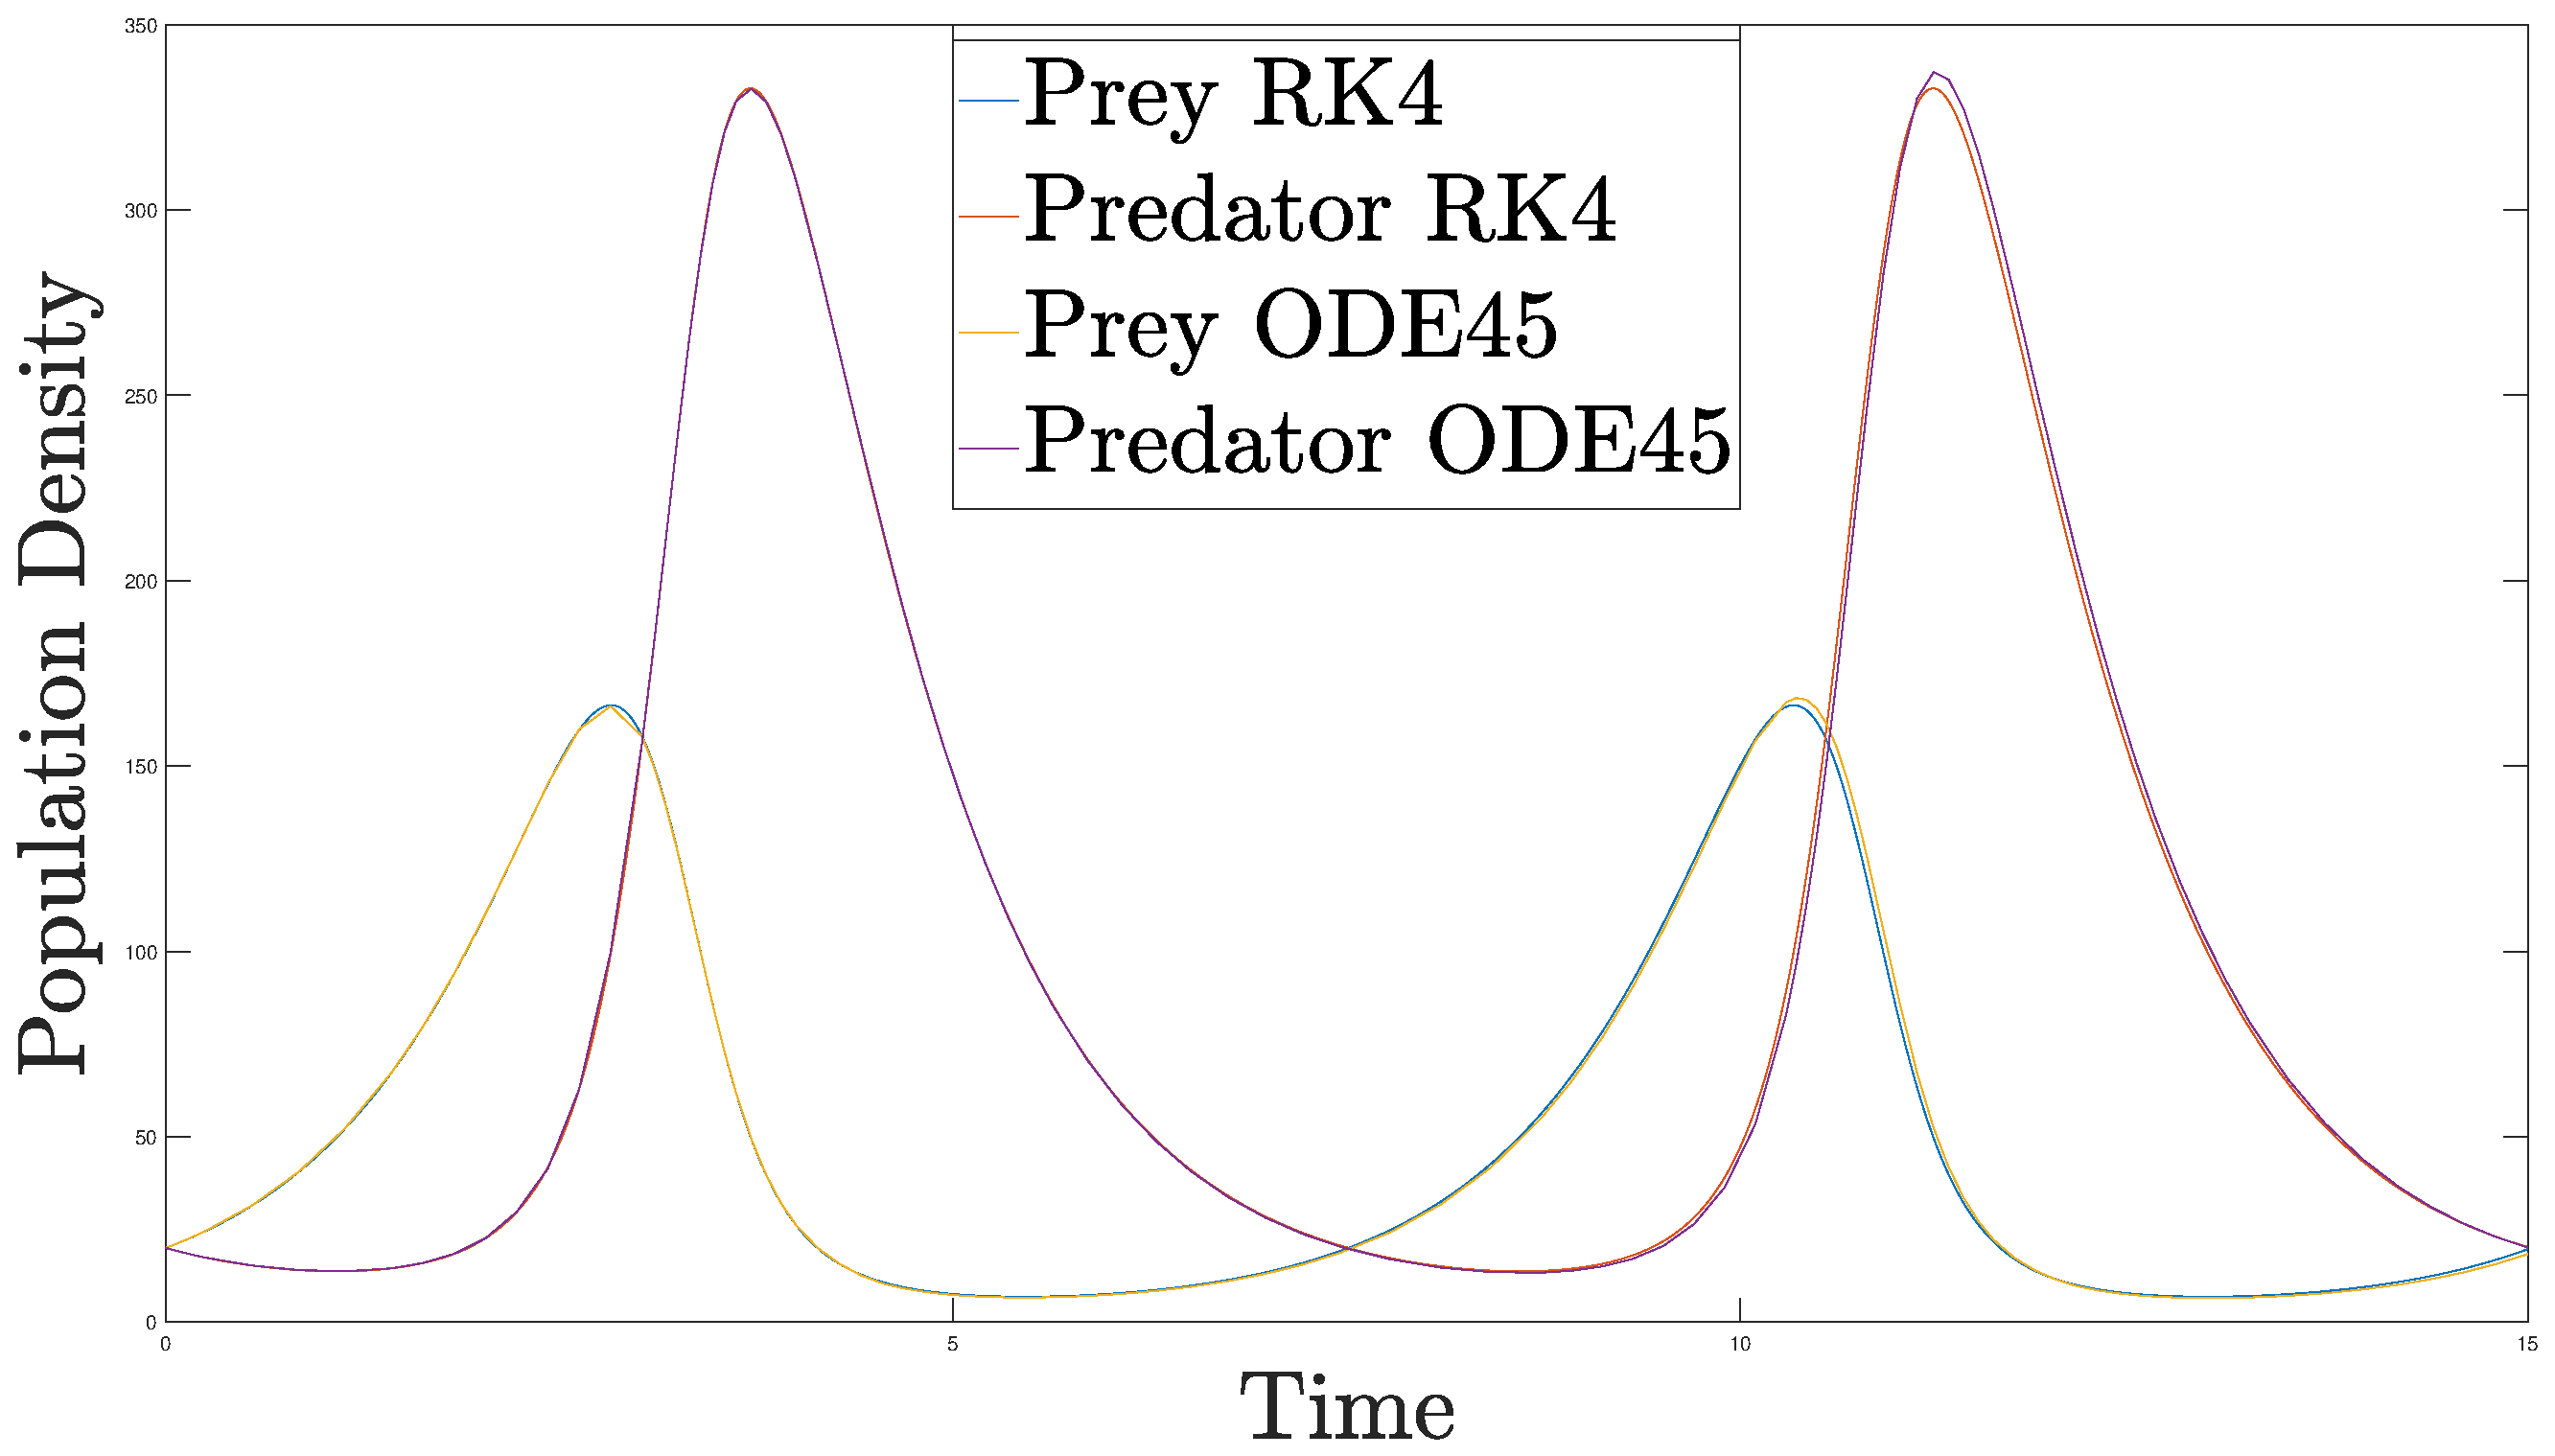
\includegraphics[width = 1\textwidth]{Images/Density.eps}
 		\caption{Predator and Prey Population Densities Over Time for Runge-Kutta \nth{4} Order and ODE45}
 		\label{fig:1}
        \end{center}
 		
\end{figure}


\begin{figure}[H]
\begin{center}
 		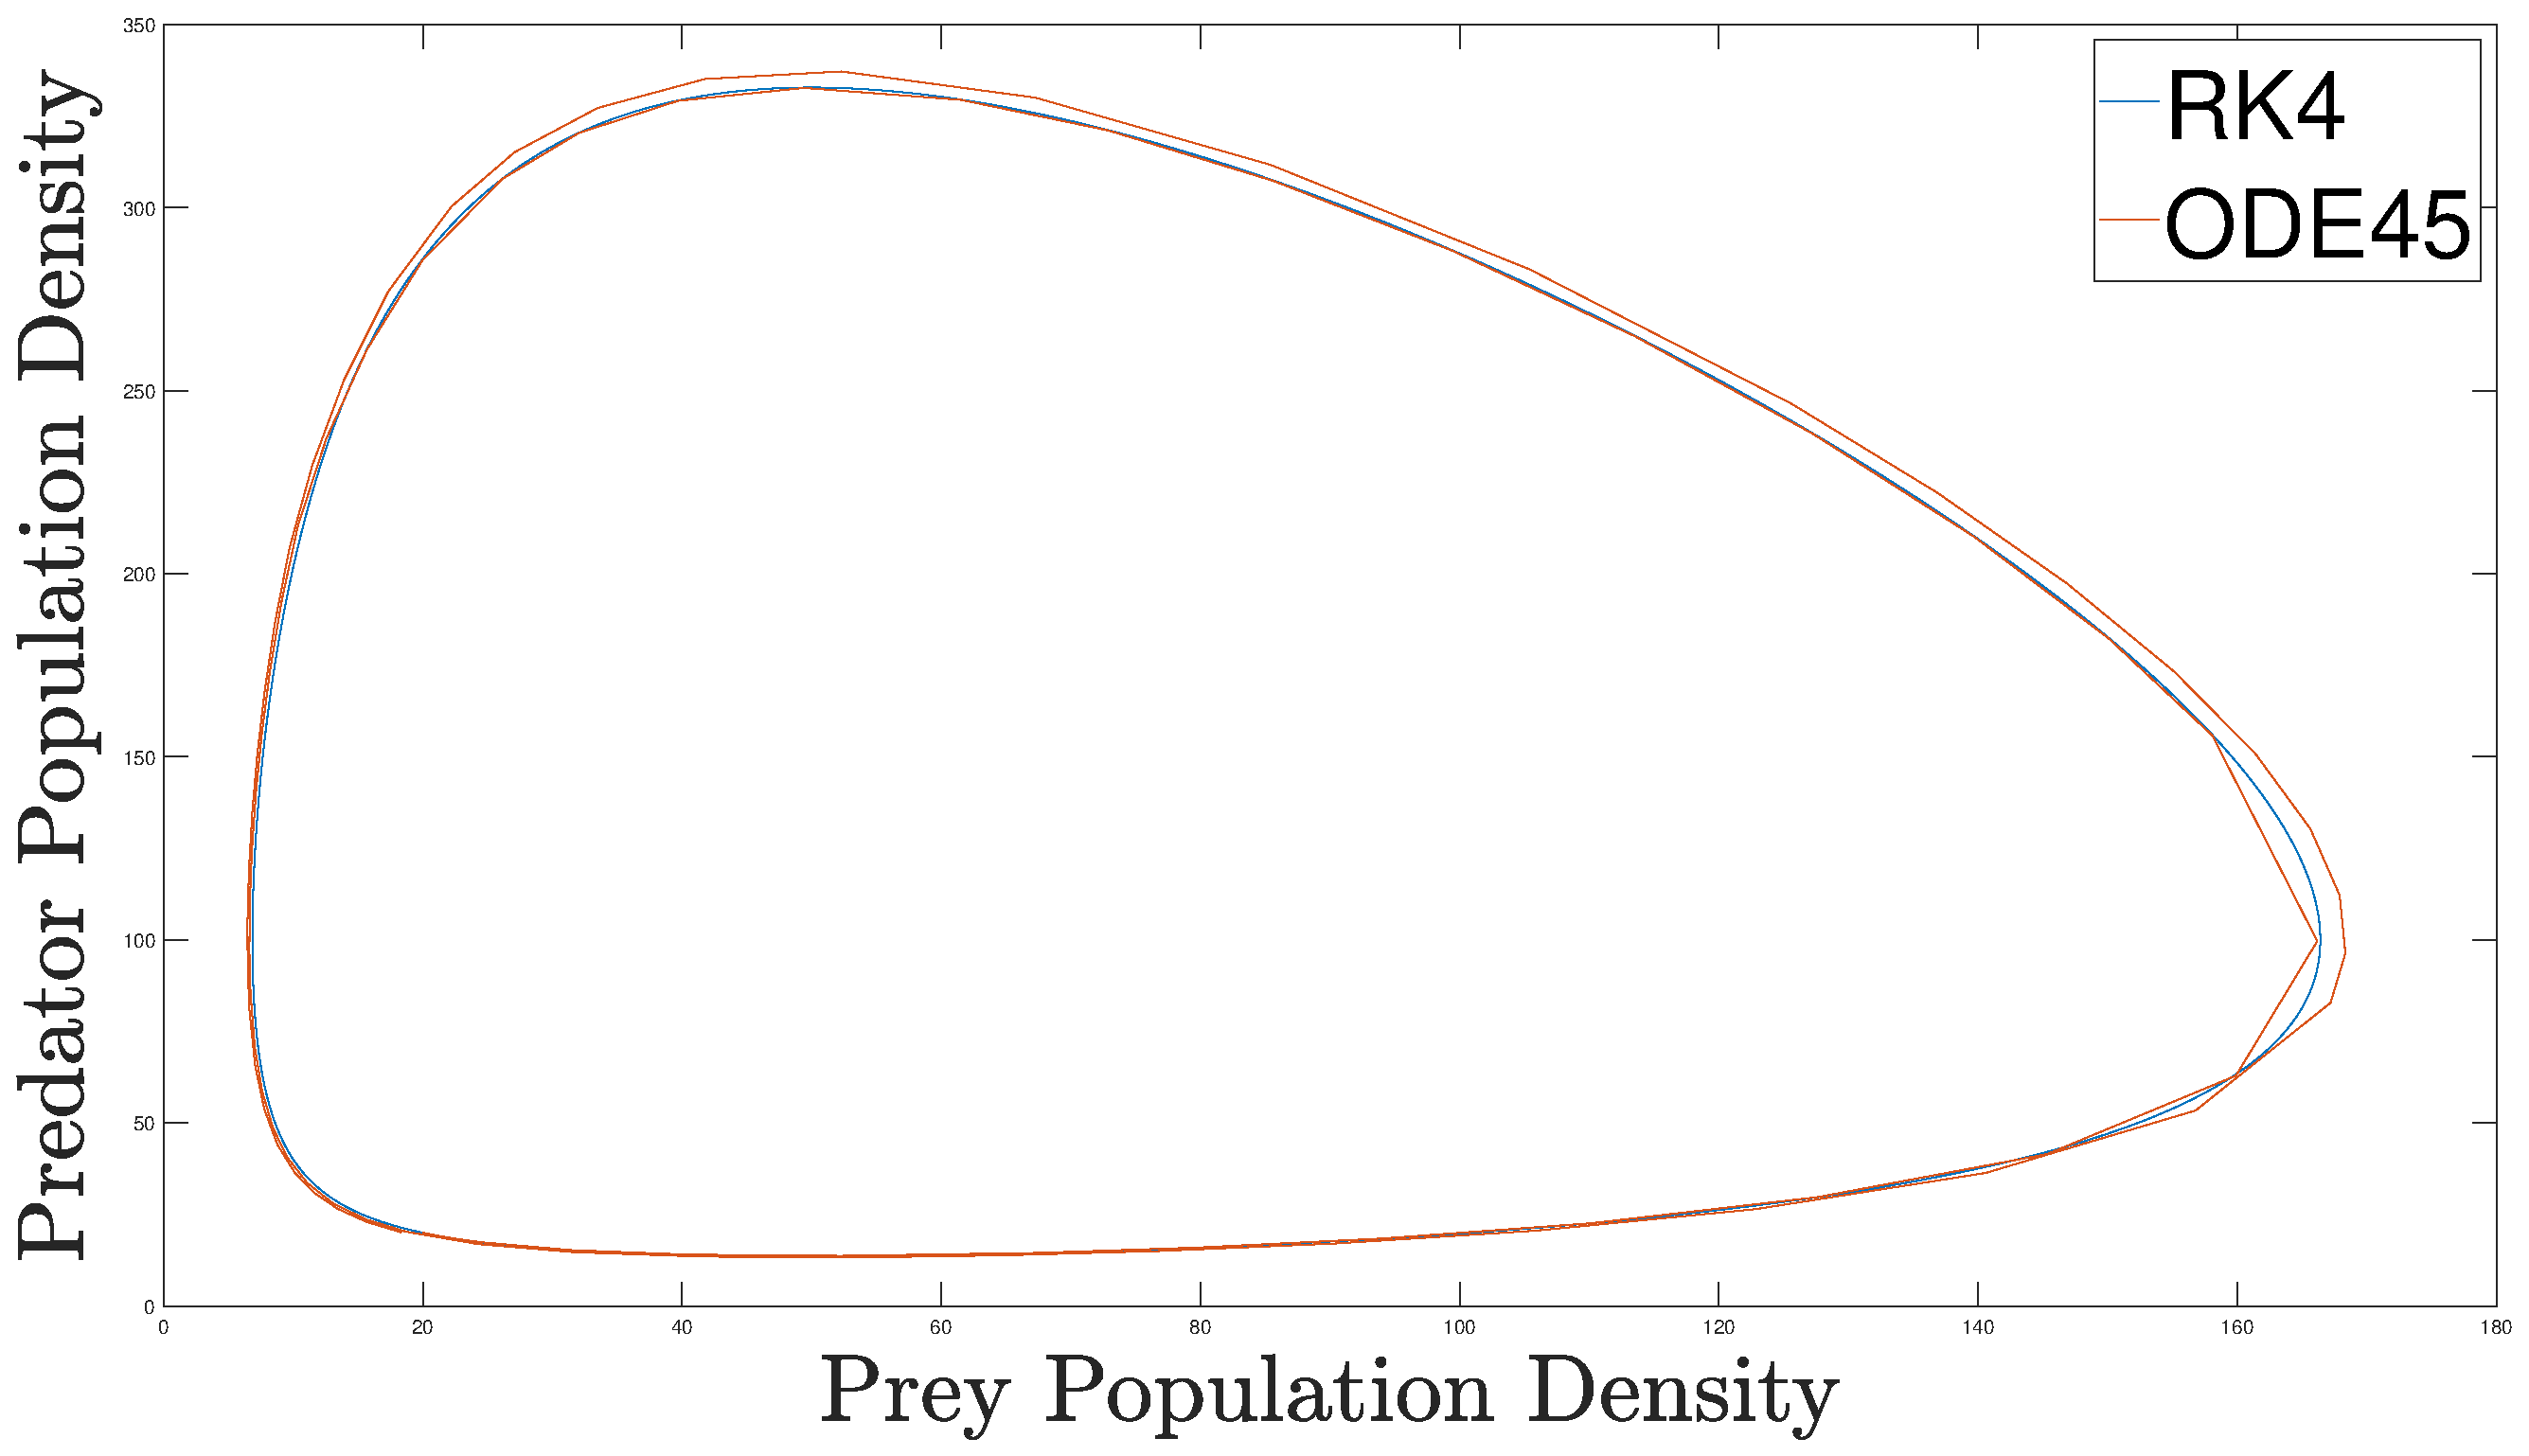
\includegraphics[width = 1\textwidth]{Images/Phase.eps}
 		\caption{Predator and Prey Phase Space between Runge-Kutta \nth{4} Order and ODE45}
 		\label{fig:2}
    \end{center}
\end{figure}
\subsubsection{Analysis of RK4 versus ODE45}
In each Figure, we can see our RK4 method is overlapping the ODE45 plots in a smoother manner, meaning our method is approximating the Lotka-Volterra Model as best as possible.
Since our approximation solution is incredibly accurate to the Lotka-Volterra Model generated by ODE45, we can confirm that our method is working as expected.

\begin{figure}[H]
    \centering
\end{figure}


% ----------------------------------------------------------------------
% Conclusion
% ----------------------------------------------------------------------
\section{Conclusion}
In summation, the Lotka-Volterra model effectively displays how predator-prey systems can be analyzed using ODE's. The results of the experiment show that our RK4 implementation of the Lotka-Volterra model is extremely close to the approximation given by ODE45. While our results were promising, our model could be improved by testing with different initial conditions and increasing the time duration. Additionally, further work can be done to test predator-prey systems with more than 2 populations or with different constraints.
\newpage
% ----------------------------------------------------------------------
% References
% ----------------------------------------------------------------------
\bibliographystyle{plain}
\bibliography{refs}
\end{document}